\documentclass{article}
%%%%%%%%%%%%%%%%%%%%%%%%%%%%% Define Article %%%%%%%%%%%%%%%%%%%%%%%%%%%%%%%%%%
%%%%%%%%%%%%%%%%%%%%%%%%%%%%%%%%%%%%%%%%%%%%%%%%%%%%%%%%%%%%%%%%%%%%%%%%%%%%%%%

%%%%%%%%%%%%%%%%%%%%%%%%%%%%% Using Packages %%%%%%%%%%%%%%%%%%%%%%%%%%%%%%%%%%
\usepackage{float}
\usepackage[letterpaper,portrait]{geometry}
\usepackage{graphicx}
\usepackage{anysize}
\usepackage{lipsum}
\usepackage{amsmath,amssymb,amsthm}
\usepackage[utf8]{inputenc}
\usepackage{multirow}
\usepackage{csquotes}
\usepackage[spanish]{babel}
\usepackage{apacite}
\usepackage{multicol}
\usepackage{parskip}
\usepackage{setspace}
\usepackage{empheq}
\usepackage{mdframed}
\usepackage{booktabs}
\usepackage{lipsum}
\usepackage{graphicx}
\usepackage{color}
\usepackage{psfrag}
\usepackage{pgfplots}
\usepackage{bm}
\usepackage{tocloft}
\usepackage{lscape}
\usepackage{adjustbox}
%%%%%%%%%%%%%%%%%%%%%%%%%%%%%%%%%%%%%%%%%%%%%%%%%%%%%%%%%%%%%%%%%%%%%%%%%%%%%%%

% Other Settings

%%%%%%%%%%%%%%%%%%%%%%%%%% Page Setting %%%%%%%%%%%%%%%%%%%%%%%%%%%%%%%%%%%%%%%
\geometry{letterpaper, margin=2.54cm}

%%%%%%%%%%%%%%%%%%%%%%%%%% Define some useful colors %%%%%%%%%%%%%%%%%%%%%%%%%%
\definecolor{ocre}{RGB}{243,102,25}
\definecolor{mygray}{RGB}{243,243,244}
\definecolor{deepGreen}{RGB}{26,111,0}
\definecolor{shallowGreen}{RGB}{235,255,255}
\definecolor{deepBlue}{RGB}{61,124,222}
\definecolor{shallowBlue}{RGB}{235,249,255}
%%%%%%%%%%%%%%%%%%%%%%%%%%%%%%%%%%%%%%%%%%%%%%%%%%%%%%%%%%%%%%%%%%%%%%%%%%%%%%%

%%%%%%%%%%%%%%%%%%%%%%%%%% Define an orangebox command %%%%%%%%%%%%%%%%%%%%%%%%
\newcommand\orangebox[1]{\fcolorbox{ocre}{mygray}{\hspace{1em}#1\hspace{1em}}}
%%%%%%%%%%%%%%%%%%%%%%%%%%%%%%%%%%%%%%%%%%%%%%%%%%%%%%%%%%%%%%%%%%%%%%%%%%%%%%%

%%%%%%%%%%%%%%%%%%%%%%%%%%%% English Environments %%%%%%%%%%%%%%%%%%%%%%%%%%%%%
\newtheoremstyle{mytheoremstyle}{3pt}{3pt}{\normalfont}{0cm}{\rmfamily\bfseries}{}{1em}{{\color{black}\thmname{#1}~\thmnumber{#2}}\thmnote{\,--\,#3}}
\newtheoremstyle{myproblemstyle}{3pt}{3pt}{\normalfont}{0cm}{\rmfamily\bfseries}{}{1em}{{\color{black}\thmname{#1}~\thmnumber{#2}}\thmnote{\,--\,#3}}
\theoremstyle{mytheoremstyle}
\newmdtheoremenv[linewidth=1pt,backgroundcolor=shallowGreen,linecolor=deepGreen,leftmargin=0pt,innerleftmargin=20pt,innerrightmargin=20pt,]{theorem}{Theorem}[section]
\theoremstyle{mytheoremstyle}
\newmdtheoremenv[linewidth=1pt,backgroundcolor=shallowBlue,linecolor=deepBlue,leftmargin=0pt,innerleftmargin=20pt,innerrightmargin=20pt,]{definition}{Definition}[section]
\theoremstyle{myproblemstyle}
\newmdtheoremenv[linecolor=black,leftmargin=0pt,innerleftmargin=10pt,innerrightmargin=10pt,]{problem}{Problem}[section]
%%%%%%%%%%%%%%%%%%%%%%%%%%%%%%%%%%%%%%%%%%%%%%%%%%%%%%%%%%%%%%%%%%%%%%%%%%%%%%%

%%%%%%%%%%%%%%%%%%%%%%%%%%%%%%% Plotting Settings %%%%%%%%%%%%%%%%%%%%%%%%%%%%%
\usepgfplotslibrary{colorbrewer}
\pgfplotsset{width=8cm,compat=1.9}
%%%%%%%%%%%%%%%%%%%%%%%%%%%%%%%%%%%%%%%%%%%%%%%%%%%%%%%%%%%%%%%%%%%%%%%%%%%%%%%

%%%%%%%%%%%%%%%%%%%%%%%%%%%%%%% Title & Author %%%%%%%%%%%%%%%%%%%%%%%%%%%%%%%%
\author{Gustavo Vergara}
%%%%%%%%%%%%%%%%%%%%%%%%%%%%%%%%%%%%%%%%%%%%%%%%%%%%%%%%%%%%%%%%%%%%%%%%%%%%%%%

\begin{document}
\pgfplotsset{compat=1.18}
\setstretch{2}

\begin{titlepage}
	\centering
	\vspace{2.5cm}
	{\scshape \Large Diagramas y documentación de actividades del proyecto - GA2-220501093-AA1-EV04 \par}
	\vspace{5cm}
	\textbf\large\scshape{\par}
	\vspace{0.5cm}

	{\Large Vergara Pareja Gustavo\par}
	\vspace{5cm}
	{\scshape\Large Jovanna Herazo\par}
	\vspace{0.3cm}
	{\scshape\Large Tecnología en Análisis y Desarrollo de Software \par}
	\vspace{0.3cm}
	{\scshape\Large SENA - Centro Agropecuario Regional Cauca\par}
	\vspace{0.3cm}
	{\Large \today \par}
\end{titlepage}

\begin{flushleft}
	\large \textbf{EVIDENCIA A SOLUCIONAR}\\
	\vspace{0.1cm}
	\section*{Evidencia GA2-220501093-AA1-EV04: diagramas y documentación de actividades del proyecto}
	Con base en los requisitos del sistema ya especificados, se empiezan a construir los artefactos del modelo necesarios para representar la solución de software, por medio de los siguientes documentos: diagramas de clase, documentos de casos de uso o historias de usuario en plantillas, modelo de base de datos, modelo del dominio, diagramas de actividades y también un documento informe con los resultados obtenidos. Aspectos a tener en cuenta:
	\begin{itemize}
		\item Estudiar detenidamente los conceptos y características definidas en el
		      componente formativo.
		\item Revisar el video sugerido como material complementario del componente
		      formativo.
		\item Manejar el lenguaje de modelado UML
		\item Manejar metodologías tipo ágil.
		\item Identificar la metodología de desarrollo a seguir.
	\end{itemize}
\end{flushleft}
\newpage
%\tableofcontents

\section{Metodología de desarrollo}
La metodología de desarrollo que se utilizará es Extreme Programming (XP). XP
es una metodología ágil que se basa en los siguientes principios:

\begin{itemize}
	\item Comunicación y Coraje: La comunicación entre los miembros del equipo es
	      fundamental para el éxito del proyecto.
	\item Feedback: El cliente debe proporcionar retroalimentación constante al equipo de
	      desarrollo.
	\item Simplicidad: El software debe ser simple de entender y mantener.
	\item Colaboración y Respeto: El equipo debe trabajar de forma colaborativa para
	      entregar el software.

\end{itemize}

Las actividades a cumplir para el desarrollo del sistema de gestión de citas
médicas se pueden dividir en las siguientes fases:
\begin{enumerate}
	\item Fase de planificación: En esta fase se define el alcance del proyecto, se
	      identifican los requisitos del sistema y se elabora el plan de desarrollo.
	\item Fase de iteraciones: En esta fase se implementa el sistema de acuerdo con los
	      requisitos definidos en la fase de planificación. Cada iteración dura
	      aproximadamente dos semanas y se divide en las siguientes actividades:
	      \begin{itemize}
		      \item   Planificación: Los equipos de desarrollo definen las tareas que se realizarán
		            en la iteración.
		      \item  Desarrollo: Los equipos de desarrollo implementan las tareas definidas en la
		            fase de planificación.
		      \item  Pruebas: Los equipos de desarrollo realizan pruebas del sistema para verificar
		            que cumpla con los requisitos.
		      \item  Revisión: Los equipos de desarrollo revisan el sistema con los usuarios para
		            obtener feedback.
		      \item Fase de implementación: En esta fase se instala el sistema en el entorno de
		            producción.
	      \end{itemize}
\end{enumerate}
\section{Diagramas}
Los diagramas presentados a continuación, son diagramas realizados con StarUML
\begin{figure}[H]
	\centering
	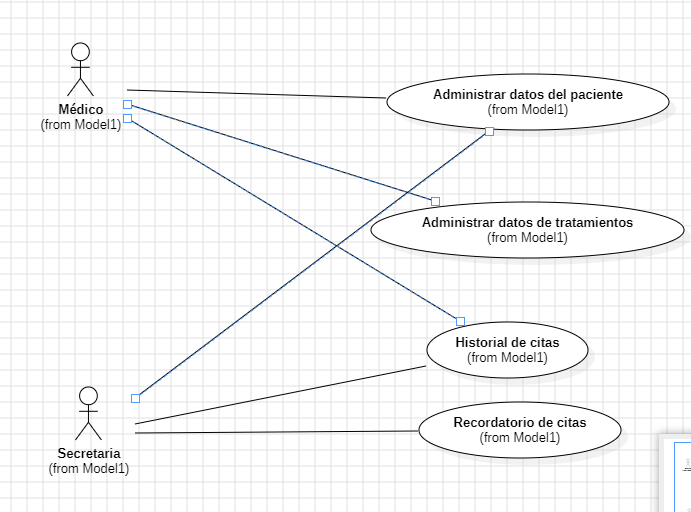
\includegraphics[width=1\textwidth]{diagrama.png}
	\caption{Diagrama de casos de uso}
	\label{fig:imagen1}
\end{figure}

\begin{figure}[H]
	\centering
	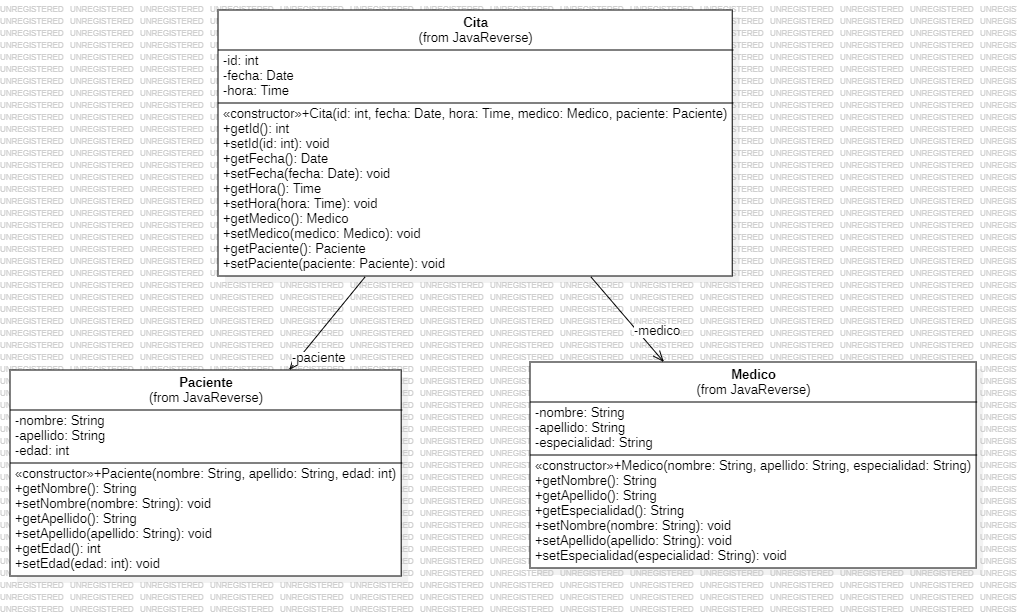
\includegraphics[width=1\textwidth]{Diagrama de clase.png}
	\caption{Diagrama de clases}
	\label{fig:imagen2}
\end{figure}
\section{Cronograma de actividades}
El documento de cronograma de trabajo del proyecto debe incluir la siguiente información:
\begin{itemize}
	\item Lista de actividades a realizar.
	\item Duración estimada de cada actividad.
	\item  Fecha de inicio y finalización de cada actividad.
	\item Equipo responsable de cada actividad.
\end{itemize}

A continuación, se presenta un ejemplo de cronograma de trabajo para el
desarrollo del sistema de gestión de citas médicas utilizando XP.
\newpage

% Contenido que se imprimirá en formato de página horizontal

%\begin{landscape} 

\begin{table}[!ht]
	\centering
	\begin{adjustbox}{max width=1.15\textwidth}
		\small
		\begin{tabular}{|l|l|l|l|l|l|}
			\hline
			**Actividad                & Duración estimada & Fecha de inicio        & Fecha de finalización  & Equipo responsable  ~       \\ \hline
			Iteración 1                & 2 semanas         & 20 de November de 2023 & 3 de December de 2023  & Equipo de desarrollo  ~     \\ \hline
			Iteración 2                & 2 semanas         & 4 de December de 2023  & 17 de December de 2023 & Equipo de desarrollo  ~     \\ \hline
			Iteración 3                & 2 semanas         & 18 de December de 2023 & 31 de December de 2023 & Equipo de desarrollo  ~     \\ \hline
			Iteración 4                & 2 semanas         & 1 de January de 2024   & 14 de January de 2024  & Equipo de desarrollo  ~     \\ \hline
			Iteración 5                & 2 semanas         & 15 de January de 2024  & 28 de January de 2024  & Equipo de desarrollo  ~     \\ \hline
			Iteración 6                & 2 semanas         & 29 de January de 2024  & 11 de February de 2024 & Equipo de desarrollo  ~     \\ \hline
			Iteración 7                & 2 semanas         & 12 de February de 2024 & 25 de February de 2024 & Equipo de desarrollo  ~     \\ \hline
			Iteración 8                & 2 semanas         & 26 de February de 2024 & 10 de March de 2024    & Equipo de desarrollo  ~     \\ \hline
			Iteración 9                & 2 semanas         & 11 de March de 2024    & 24 de March de 2024    & Equipo de desarrollo  ~     \\ \hline
			Iteración 10               & 2 semanas         & 25 de March de 2024    & 7 de April de 2024     & Equipo de desarrollo  ~     \\ \hline
			Iteración 11               & 2 semanas         & 8 de April de 2024     & 21 de April de 2024    & Equipo de desarrollo  ~     \\ \hline
			Iteración 12               & 2 semanas         & 22 de April de 2024    & 5 de May de 2024       & Equipo de desarrollo  ~     \\ \hline
			Iteración 13               & 2 semanas         & 6 de May de 2024       & 19 de May de 2024      & Equipo de desarrollo  ~     \\ \hline
			Iteración 14               & 2 semanas         & 20 de May de 2024      & 2 de June de 2024      & Equipo de desarrollo  ~     \\ \hline
			Implementación del sistema & 4 semanas         & 6 de June de 2024      & 27 de June de 2024     & Equipo de implementación  ~ \\ \hline
			Pruebas del sistema        & 2 semanas         & 28 de June de 2024     & 11 de July de 2024     & Equipo de pruebas  ~        \\ \hline
			Implementación del sistema & 1 semana          & 12 de July de 2024     & 18 de July de 2024     & Equipo de implementación  ~ \\ \hline
		\end{tabular}
	\end{adjustbox}
\end{table}
\textbf{Cambios en el cronograma de trabajo}

El cronograma de trabajo puede cambiar a medida que avanza el proyecto. Estos cambios pueden ser necesarios debido a factores como:
\begin{itemize}
	\item Cambios en los requisitos del sistema.
	\item Problemas técnicos.
	\item Cambios en el entorno del proyecto.
\end{itemize}


%\end{landscape}


\end{document}
